\chapter{Deciphering microscopic drivers of viral genome-scale molecular clock dynamics}

\begin{flushright}
    \textit{Nothing in biology makes sense except in the light of evolution.}\\
    --- Theodosius Dobzhansky
\end{flushright}

\vspace{1cm}

\noindent This work has been sent to a peer-reviewed journal.\\

\noindent \textbf{Goiriz L}, Rodrigo G. (2025) {Deciphering microscopic drivers of viral genome-scale molecular clock dynamics}. \textit{Under review}.\\

\noindent In this work, I performed all the data analysis and figures. The results were discussed with GR. GR designed the research.

\vfill

\pagebreak

\sloppy

\section{Introduction}
Viruses, and in particular RNA viruses, with their short generation times and high mutation rates, offer a unique window into the dynamics of evolution \cite{elena2007virus}. Unlike in many organisms, the mutation accumulation process in viruses can be observed in real time, making them ideal systems for studying the mechanisms that drive genetic variation. By analyzing viral genomes, we can test evolutionary theories, such as neutral theory \cite{gojobori1990molecular} or lethal mutagenesis \cite{crotty2001rna}, we can track how mutations spread through populations \cite{kraemer2021spatiotemporal,viana2022rapid}, which results in a critical tool in epidemiology to propose suitable interventions, and we can ultimately assess how selection, drift, and recombination shape genetic diversity \cite{nelson2006stochastic,tully2009shifts}. However, viruses do not evolve uniformly across their genomes. They contain several genes coding for different types of proteins (e.g., structural and non-structural), each subject to singular selection pressures that shape its evolution rate and variability \cite{gray2011mode}. For example, genes encoding instrumental proteins to generate progeny [e.g., capsid or RNA-dependent RNA polymerase (RdRp)] tend to evolve more slowly due to strong purifying selection, while genes encoding proteins involved in direct interactions with host cell elements (e.g., glycoproteins with receptor-binding domains) are usually subject to positive selection \cite{kistler2022rapid}. In this regard, further research is needed to determine the precise contribution of each gene, which may additionally change with time, to the evolution of a virus as a whole entity.

Evolutionary processes are often described using stochastic models that assume regularity in the accumulation of genetic changes. The molecular clock hypothesis is a traditional theoretical framework derived from neutral theory that has provided foundational insights into diversification by relying on the assumption that mutations accumulate at a relatively constant rate over time and that the extent of variability in a population follows a Poisson distribution \cite{kimura1987molecular,kumar2005molecular}. Despite the wide application of this model, virus evolution can deviate from its predictions due to factors such as transmission bottlenecks, host immune pressures (e.g., vaccination), and environmental changes \cite{jenkins2002rates}. In this regard, relaxed molecular clock descriptions have been developed to allow evolution rates to vary among phylogenetic tree branches, thereby accommodating the potential effects of external factors \cite{drummond2006relaxed}. In these models, however, variation is always driven by delta-correlated (white) Gaussian noise to end with Poissonian statistics. We can then consider that each gene from a virus evolves at a given rate displaying a distinctive level of variation and that the integration of the different dynamics results into the observed evolutionary movement of the virus \cite{neher2022contributions}. Disentangling the overlooked statistical properties that characterize such individual dynamics is important for a fundamental understanding of the process and requires further introspective analysis of high-throughput sequencing data. 

The global public health crisis provoked by the emergence of severe acute respiratory syndrome coronavirus 2 (SARS-CoV-2; \cite{wu2020new}) prompted the implementation of genomic surveillance programs. It is therefore appealing to focus the study on this RNA virus to take advantage of the resulting database with millions of whole genome sequences. Notably, such efforts facilitated the detection of novel variants of concern \cite{viana2022rapid}, as well as the spatiotemporal monitoring of the impact of introduction and superspreading events \cite{kraemer2021spatiotemporal,lemieux2021phylogenetic}. They have also allowed the quantification of the interplay between adaptation, neutrality, and purifying selection during virus evolution in nature at an unprecedented resolution \cite{neher2022contributions,markov2023evolution}. In particular, it has been shown that rapid bursts of adaptation were followed by phases of slow evolution in which purifying selection predominated. Moreover, we have pointed out that each variant evolved at a different rate and that the observed genetic variability is compatible with a stochastic anomalous diffusion process (viz., with time-dependent Gaussian noise) distinctively parameterized in each case \cite{goiriz2023variant}. This indicates deviations from Poissonian statistics and highlights evolutionary constraints associated with each genotype. Notwithstanding, the mechanisms underlying this anomalous diffusion behavior remain unknown. 

In this work, we analyze the gene-level mutational dynamics of SARS-CoV-2 to determine how microscopic contributions shape macroscopic evolutionary trends. For that, we focus on the different within-variant evolution phases and quantify for each gene the process of mutation accumulation and the generation of variability. More specifically, we calculate the mean number of accumulated mutations, the mutational variance of the population, and the frequency of each mutation to provide a comprehensive evolutionary picture for each of the 27 genes of SARS-CoV-2 \cite{yang2021structural} (ORF3b and ORF9c were discarded in our study). We aim to identify whether specific genes show deviations from the classical molecular clock predictions and how these local effects drive the anomalous diffusion behavior reported at the genome-scale level. Unraveling these complexities might also enhance our ability to predict virus evolution \cite{rouzine2001transition}, with implications in epidemiology. To effectively process a massive number of genomic sequences, we here follow a statistical approach \cite{obermeyer2022analysis,goiriz2023variant}, examining population genetic compositions over time rather than reconstructing phylogenetic trees from genetic variation. Conventional phylogenetic methods \cite{bouckaert2014beast} show great utility to track pathogen evolution in public health crisis scenarios in order to e.g. identify mutations that increase fitness and to trace transmission routes (especially when mobility data are aggregated; \cite{kraemer2021spatiotemporal}). However, they do not directly follow the genetic shaping of the population through characteristic statistical parameters (moments, frequencies) and highly depend on proper prior selection; in addition to struggling with scalability due to an excessive computational demand, thereby becoming unpractical or requiring approximations when dealing with a vast number of sequences \cite{demaio2023maximum}. Through this top-down approach from large empirical observations, we seek to refine probabilistic models of viral genome evolution under the molecular clock prism and further appreciate the complexity of the mutation-selection process in infectious agents circulating in nature.

\section{Results}
We implemented a simple-method computational pipeline to process the massive number of available SARS-CoV-2 whole genome sequences and extract time-dependent statistical parameters characterizing the evolutionary trajectory of the virus. We mainly focused our analysis on the United Kingdom (UK) during the first 120 weeks of pandemic, because a strong genomic surveillance program was implemented in this geographic region at that time \cite{coguk2020integrated}. After curating the available dataset to remove poor-quality, non-date-annotated, and outlier items, we obtained 1.87 million high-quality genome sequences. With respect to the reference sequence from Wuhan (China), we identified 108,347 different mutations distributed throughout the virus genome during those 120 weeks, including substitutions, insertions, and deletions (indels). During this period, new variants of concern emerged (Alpha, Delta, and Omicron), which invaded the population one after another as a consequence of acquiring distinct mutations that enhanced their transmissibility and immune evasion capabilities \cite{tao2021biological}.

A temporal representation of the mean number of accumulated mutations by gene pointed out to PLpro (encoding a protease for polyprotein processing), RdRp (encoding the replicase), S (encoding the spike protein for viral entry), and N (encoding the nucleocapsid) as the most evolved genes since the pandemic origin (\textbf{Fig. \ref{fig:fig4.1}a}). ORF9b also appeared as evolved as it overlaps with N \cite{yang2021structural}. With the emergence of Omicron, S separated from the rest of genes in terms of divergence. Other genes started to evolve with the emergence of variants, such as ORF8 with Alpha, nsp4, nsp6, and ORF7a with Delta, and M and ORF6 with Omicron. In addition, a representation of the dispersion index of the virus population by gene, calculated as the ratio between the mutational variance and mean \cite{gillespie1984molecular}, yielded a mosaic-like picture (\textbf{Fig. \ref{fig:fig4.1}b}).

\begin{figure}[ht!]
    \centering
    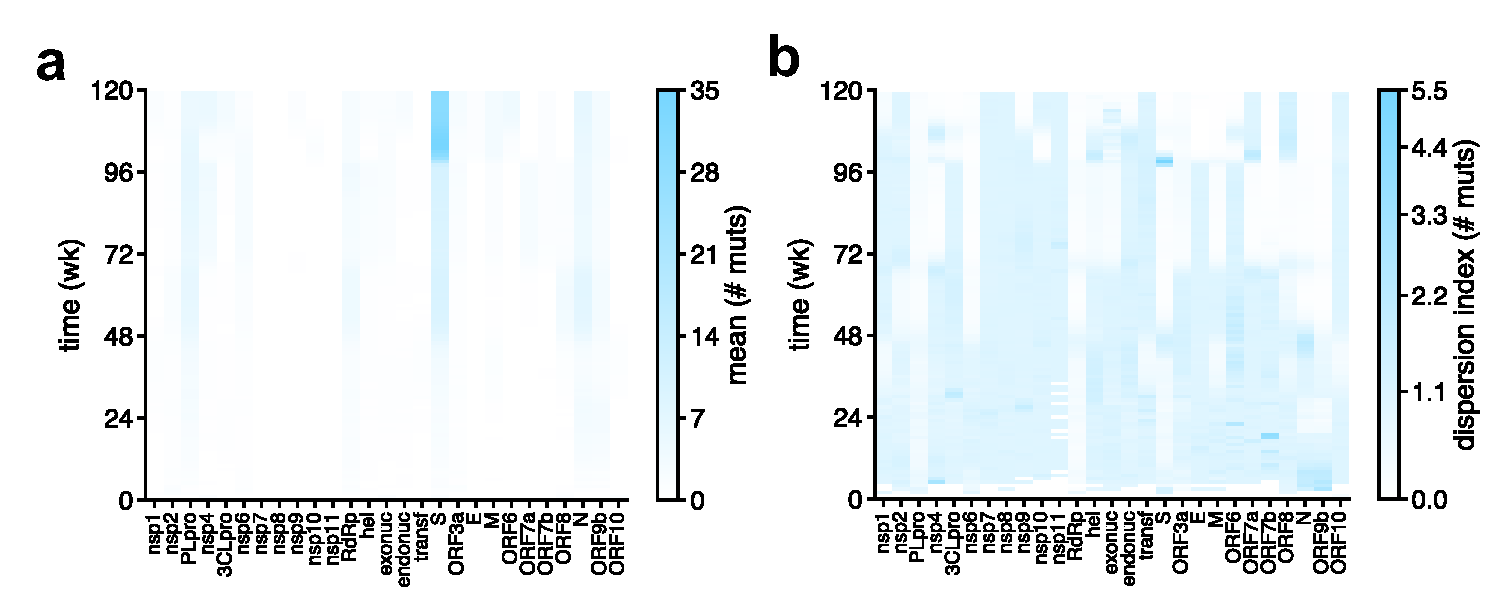
\includegraphics[width=\linewidth]{assets/Ch4Fig1.pdf}
    \caption{a) Time-course of the mean number of accumulated mutations in each gene of the SARS-CoV-2 genome, including substitutions and indels (with respect to the reference sequence from Wuhan; data from the UK). Heatmap colored using a linear scale. b) Time-course of the dispersion index (variance-to-mean ratio) of accumulated mutations in each gene of the SARS-CoV-2 genome. Heatmap colored using an inverse hyperbolic sine scale.}\label{fig:fig4.1}
\end{figure}

Non-monotonous variations in dispersion index indicate complex evolutionary trajectories, beyond deviations from Poissonian statistics. The highest genetic dispersion occurred in S with the invasion of Omicron BA.1, in agreement with multiple introductions of different sublineages in the UK \cite{tsui2023genomic}. Despite having significant evolution rate, RdRp continuously displayed reduced levels of dispersion, which could be a signature of purifying selection in order to maintain an efficient viral replication. Moreover, during the period in which Delta was the dominant variant, the dispersion in several genes was substantially low, reflecting a founder effect.

Overall, SARS-CoV-2 evolved through adaptation in a punctuated manner by accumulating non-synonymous mutations (\textbf{Fig. \ref{fig:fig4.2}a}). However, while the emergence and invasion of Alpha and Omicron BA.1 entailed bursts of non-synonymous mutations (at weeks 44 and 99, respectively), with Delta the number of non-synonymous substitutions was roughly maintained and the synonymous substitutions significantly decreased (at week 66). The dispersion index peaks ($>$ 1) clearly supported this view of the transitions (\textbf{Fig. \ref{fig:fig4.2}b}; see also the dispersion index calculated for genes encoding structural and non-structural proteins in \textbf{Fig. \ref{fig:fig4.2}c}). This is in tune with an independent emergence of Alpha and Delta in late 2020, noting that Delta first spread in India and then was introduced in the UK. Inferences of the evolution rates by gene and mutation type revealed the inclination of S, E, N, ORF7a, and exonuc to incorporate non-synonymous changes (a signature suggesting adaptation). For example, mutations H655Y and T95I in S, T9I in E, and P13L in N have been highly ranked in terms of their positive effect on viral fitness \cite{obermeyer2022analysis}. Inferences also showed that nsp9 and nsp10 preferentially accumulated synonymous mutations (a signature of purifying selection), and that nsp6 and ORF8 preferentially accumulated indels (\textbf{Fig. \ref{fig:fig4.2}d}). It has been proposed that ORF8 knockout contributes to increase viral fitness, although this may depend on the genetic background \cite{wagner2024positive}.

\begin{figure}[ht!]
    \centering
    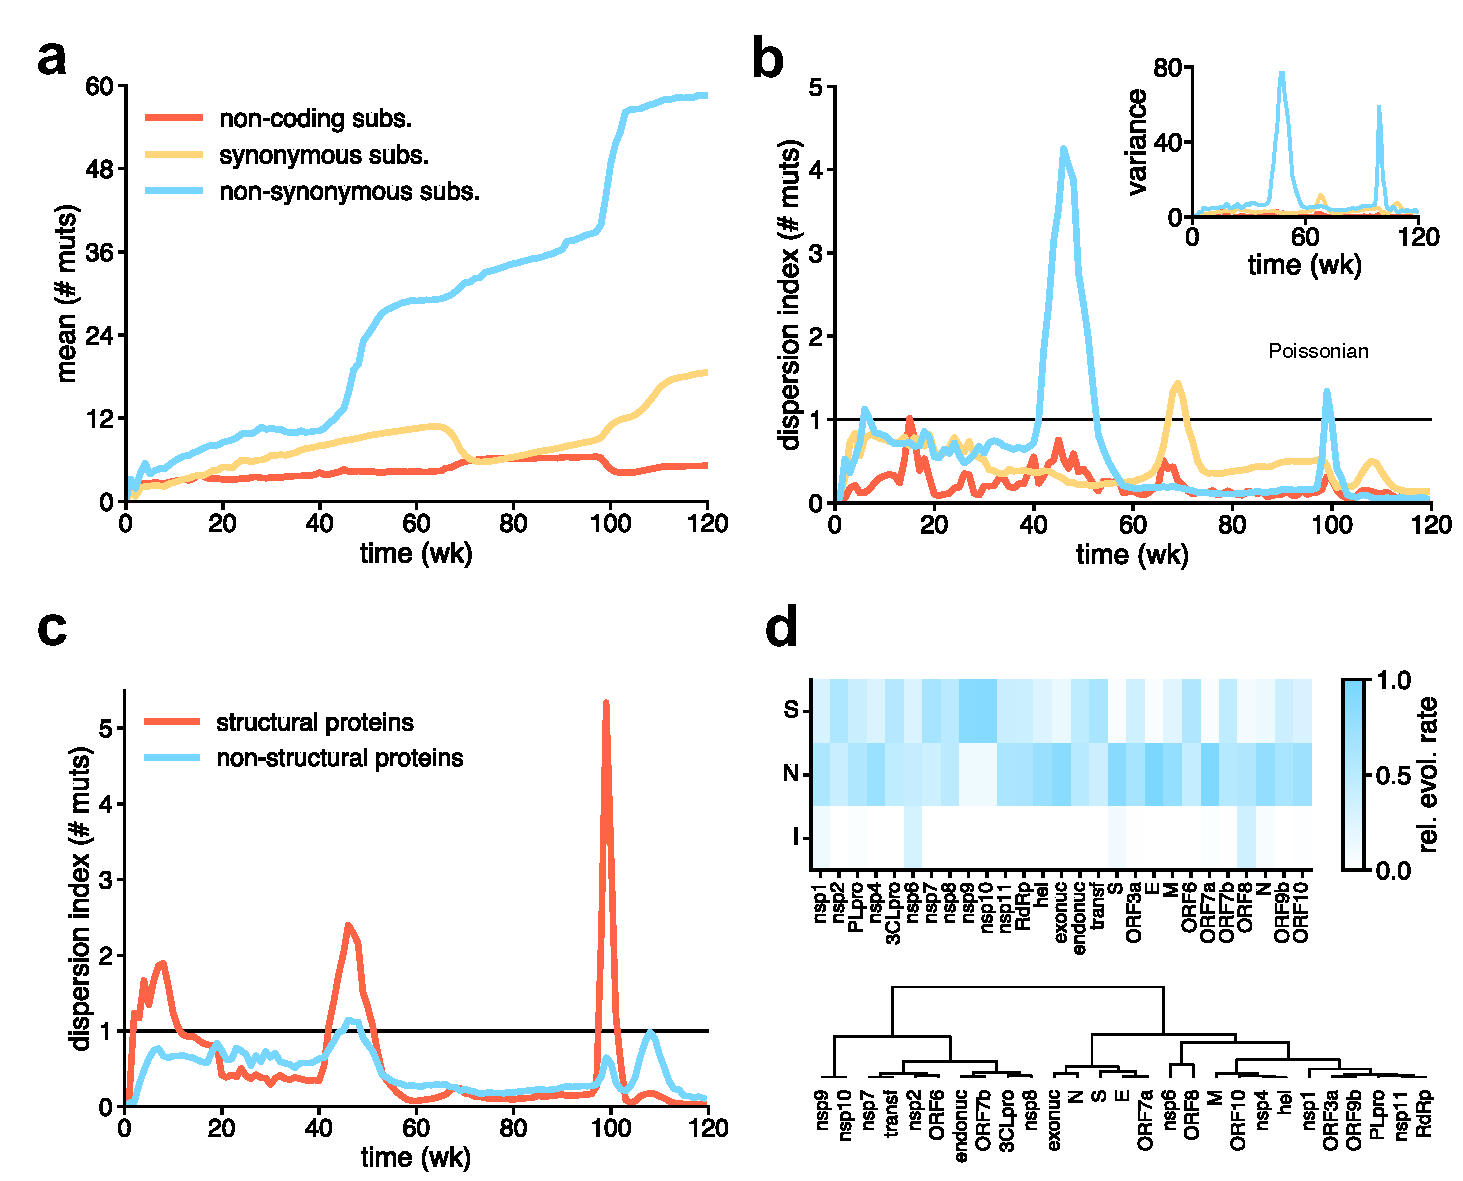
\includegraphics[width=\linewidth]{assets/Ch4Fig2.pdf}
    \caption{a) Time-course of the mean number of non-coding, synonymous, and non-synonymous substitutions. b) Time-course of the dispersion index of non-coding, synonymous, and non-synonymous substitutions. Inset, variance of substitutions with time. c) Time-course of the dispersion index in genes encoding structural and non-structural proteins. d) Inferred relative evolution rate for each gene and mutation type [synonymous substitutions (S), non-synonymous substitutions (N), and indels (I)]. Bottom, hierarchical clustering of genes.}\label{fig:fig4.2}
\end{figure}

We also analyzed the number of accumulated mutations in each gene from datasets of other countries [viz., the United States of America (USA), Spain, India, South Africa, and Japan]. Comparing the inferred evolution rates, we found similar dynamics overall (\textbf{Fig. \ref{fig:fig4.3}a}). Furthermore, we observed an interesting relationship between mutational mean and variance at particular times strictly dominated by a single variant in the UK. Considering the absolute number of mutations in each gene, Poissonian statistics hold in the case of low mutational load, being sub-Poissonian otherwise. Nevertheless, all late-stage mutational distributions get closer to the Poissonian regime by accounting for the founder effect (\textbf{Fig. \ref{fig:fig4.3}b}). Together, these results highlight the non-homogeneous genetic modulation of the virus and encourage further investigation at the variant level to completely decipher the evolutionary role of each gene.

\begin{figure}[ht!]
    \centering
    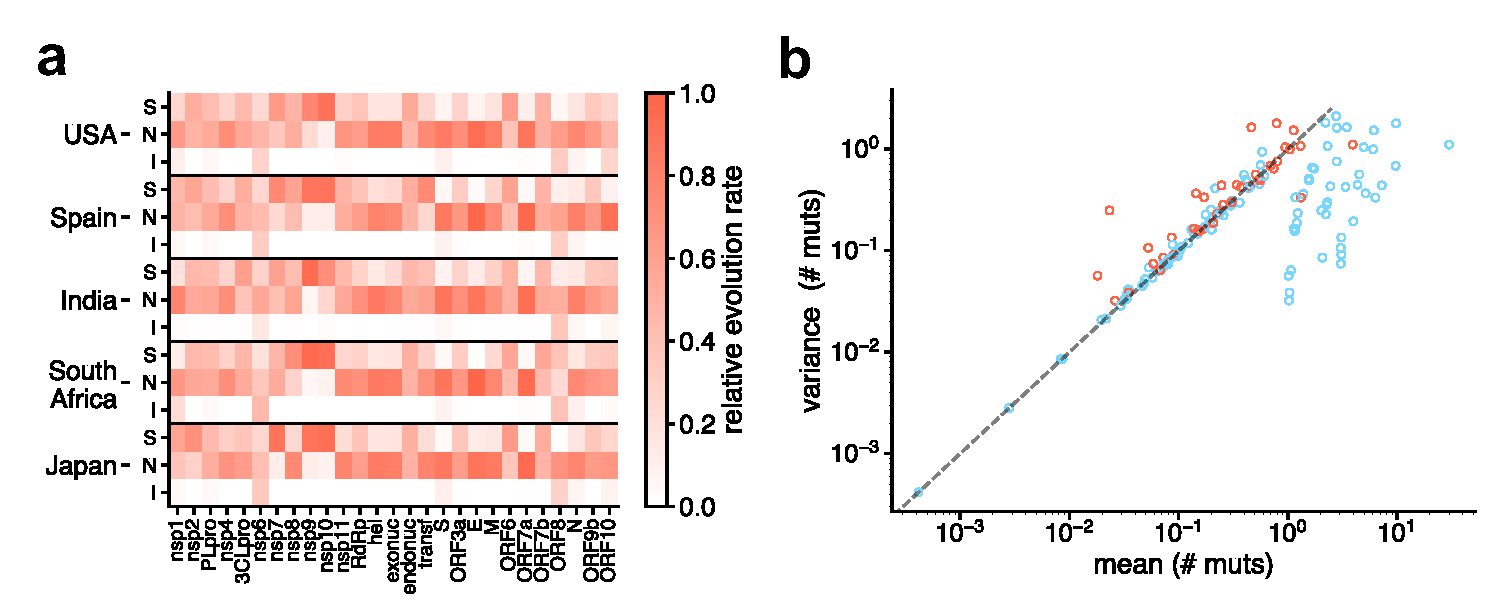
\includegraphics[width=\linewidth]{assets/Ch4Fig3.pdf}
    \caption{a) Inferred relative evolution rate for each gene and mutation type in different countries. b) Scatter plot between mean and variance in each gene at different weeks (1, 30, 60, 90, and 119). Dashed line corresponds to equal variance and mean (i.e., Poissonian regime).}\label{fig:fig4.3}
\end{figure}

According to our previous work, the whole genome of the virus accrued mutations at a nearly linear rate when particularizing for a given variant after emergence \cite{goiriz2023variant}, as predicted by the traditional molecular clock model. However, by analyzing the mean mutational load of each gene, we observed widely different dynamics (note that to ensure high statistical power, we restricted the analysis to the time window in which each variant represented at least 10\% of the population). While linear trends could be observed in various cases, we also found genes displaying highly non-linear mutation accumulation and even genes with non-monotonous and decreasing trends (\textbf{Fig. \ref{fig:fig4.4}}). The analysis of the genetic variability observed in the populations of the distinct variants also revealed intriguing microscopic aspects of the evolutionary movement of the virus, noting that an empirical model with a power law relationship between time and variance better explains the genomic data \cite{goiriz2023variant}. As in the case of the mean, non-linear, non-monotonous, and decreasing trends were found when computing the variance of the number of mutations for the different genes (\textbf{Fig. \ref{fig:fig4.5}}).

\begin{figure}[ht!]
    \centering
    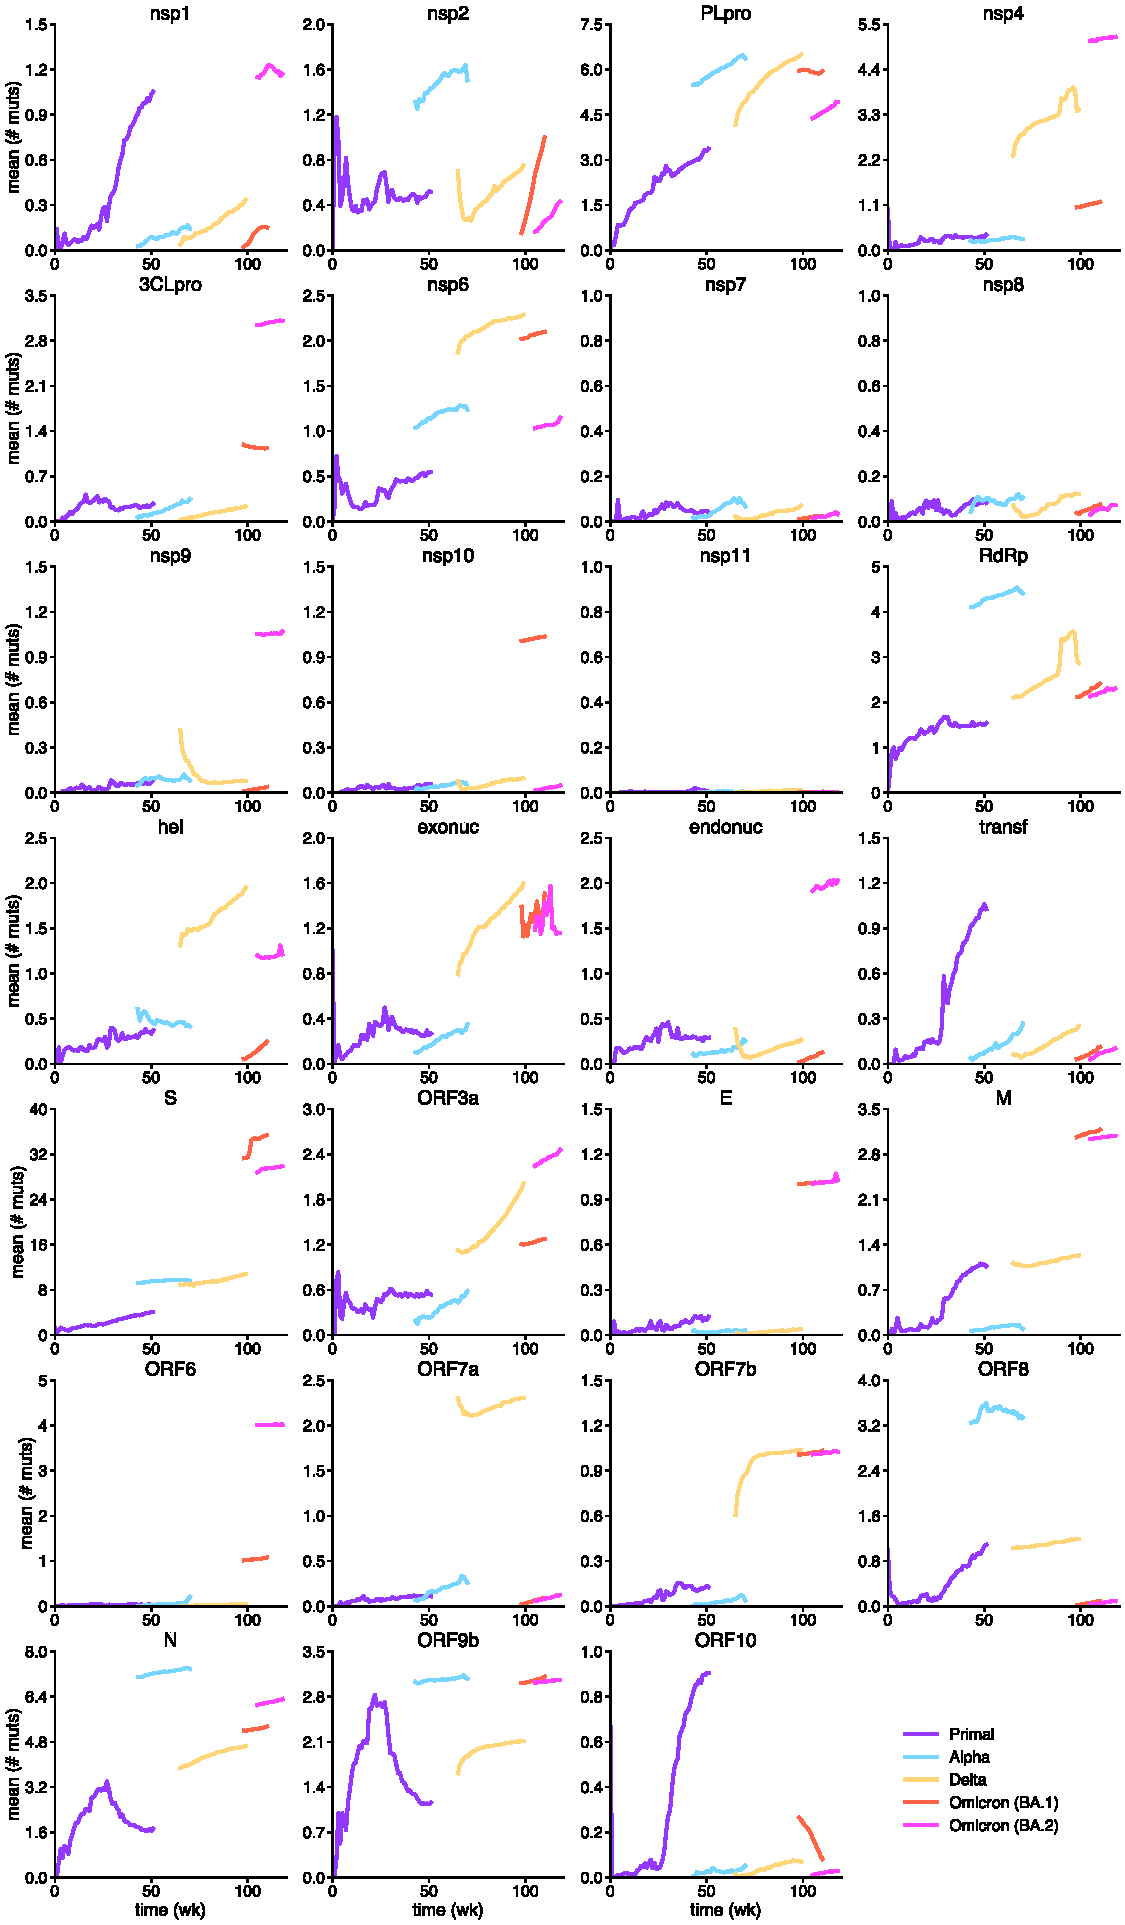
\includegraphics[width=0.7375\linewidth]{assets/Ch4Fig4.pdf}
    \caption{Gene-by-gene analysis of the variant-specific evolutionary trajectory of SARS-CoV-2. Time-course of the mean number of accumulated mutations in each gene of the SARS-CoV-2 genome and for each variant (Primal, Alpha, Delta, and Omicron BA.1 and BA.2). Mutations included substitutions and indels (with respect to the reference sequence from Wuhan; data from the UK). Analysis restricted to the time period in which the population frequencies of the variants were at least 10\%.}\label{fig:fig4.4}
\end{figure}

\begin{figure}[ht!]
    \centering
    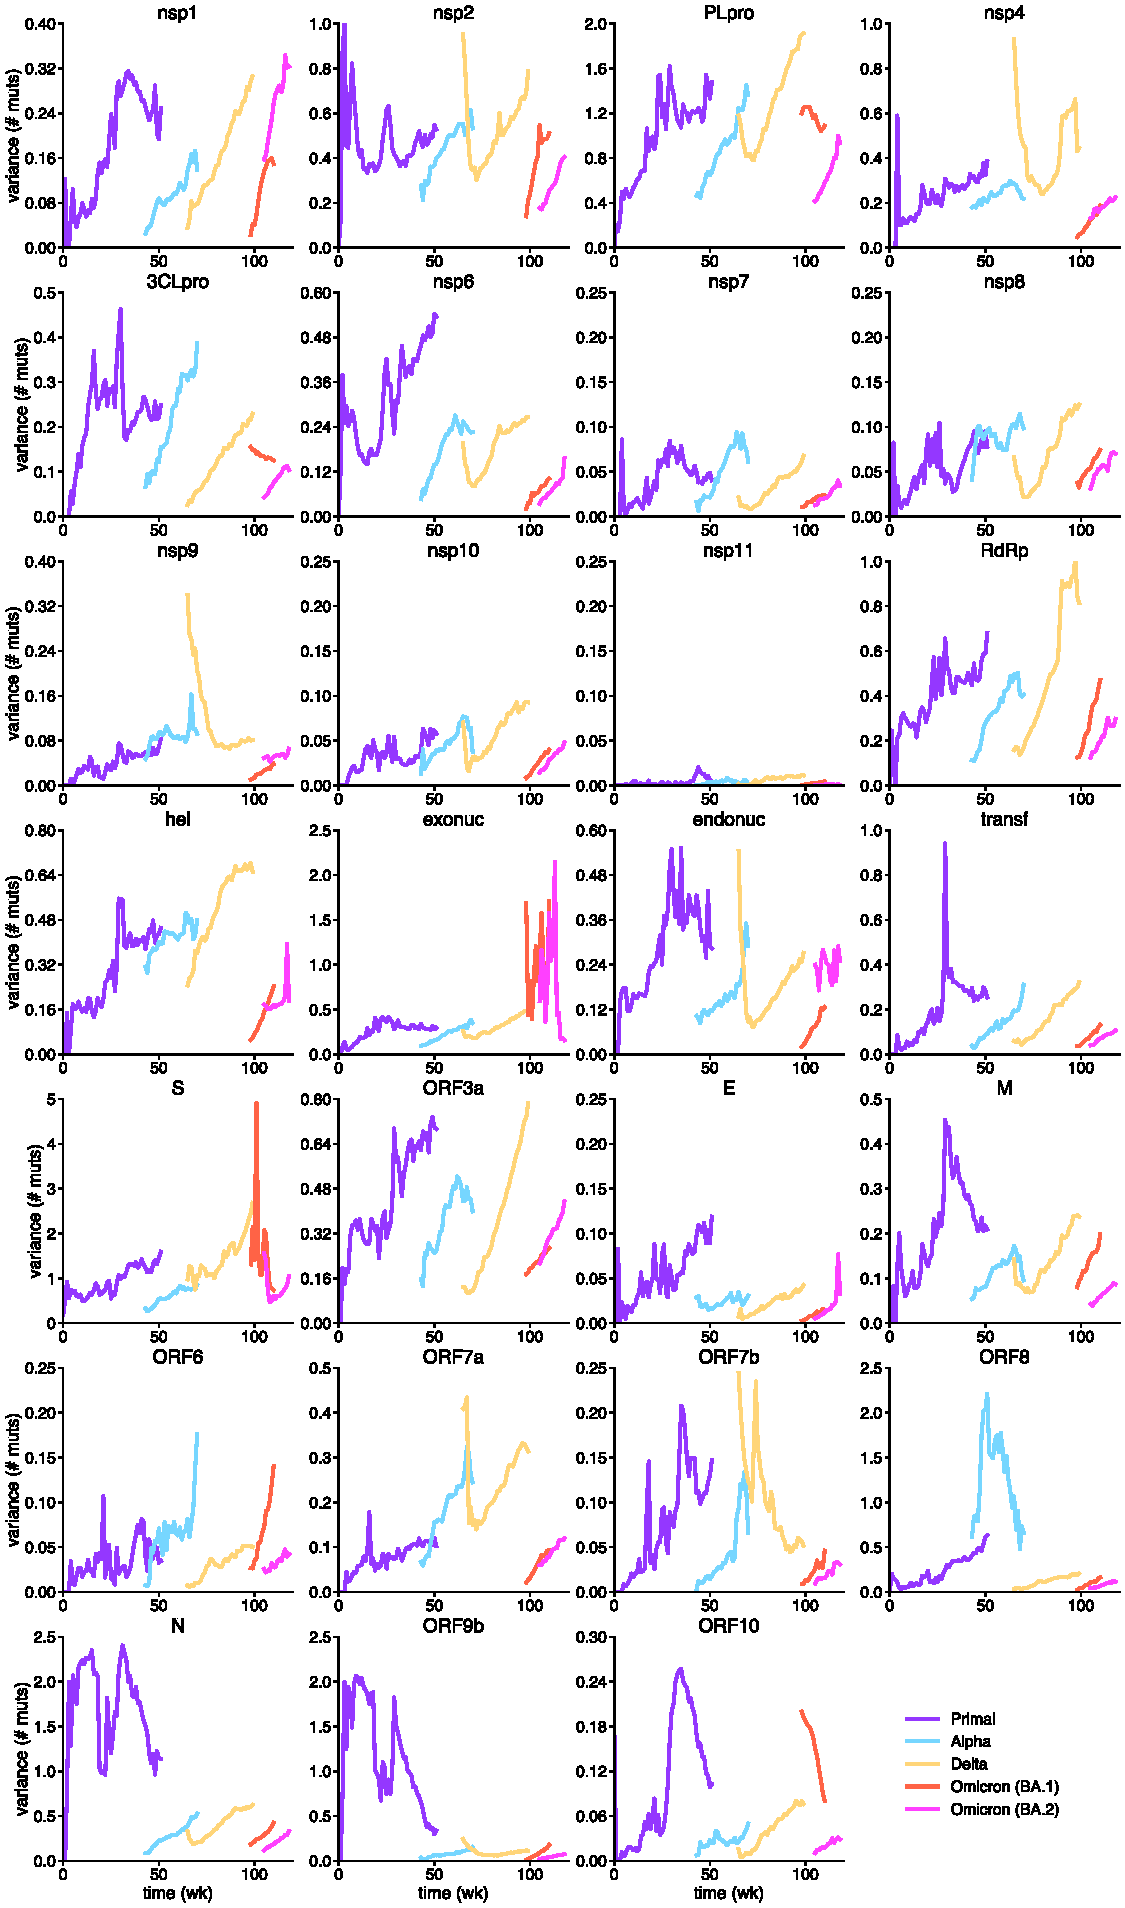
\includegraphics[width=0.7375\linewidth]{assets/Ch4Fig5.pdf}
    \caption{Gene-by-gene analysis of the variant-specific evolutionary diffusion of SARS-CoV-2. Time-course of the variance of accumulated mutations in each gene of the SARS-CoV-2 genome and for each variant (Primal, Alpha, Delta, and Omicron BA.1 and BA.2). Mutations included substitutions and indels (with respect to the reference sequence from Wuhan; data from the UK). Analysis restricted to the time period in which the population frequencies of the variants were at least 10\%.}\label{fig:fig4.5}
\end{figure}

\vfill
\pagebreak

\section{Conclusions}
Here, we have examined the microscopic factors that drive the genome-scale molecular clock dynamics of SARS-CoV-2, capitalizing on the unprecedented quantity of high-resolution sequencing data. By dissecting the virus' genome into its constituent genes, we uncovered strong non-uniformity in the patterns of mutation accumulation, highlighting the mosaic-like nature of SARS-CoV-2 evolution. Although global, genome-wide analyses reveal an overall quasi-linear accumulation of mutations at the variant level, consistent with certain predictions of the molecular clock framework, gene-level investigations reveal that specific loci often deviate from canonical Poissonian behaviors. Critically, some genes displayed highly non-monotonous or even decreasing trends in both mean mutational load and variance, underscoring the importance of local selection pressures, functional constraints, and founder effects in shaping evolutionary outcomes.

Our findings show that genes encoding essential viral functions, such as those involved in replication (RdRp) or structural integrity (N, S, and M), exhibit distinct evolutionary trajectories, reflecting a delicate balance between purifying selection and bursts of adaptive mutations. This dynamic is further evidenced by the shifts in dispersion indices through time: while some genes remain under tightly constrained evolution due to critical functional requirements (e.g., RdRp), others, particularly those facing strong interactions with host immune elements, undergo episodic bursts of adaptation (e.g., S). For instance, the non-monotonous or even decreasing mutation trajectories observed in certain genes likely result from transient selective sweeps or founder events that reset local genetic diversity, illustrating how chance transmission bottlenecks can temporarily invert or slow evolutionary trends at specific loci \cite{markov2023evolution}. Importantly, our approach leverages a statistical “top-down” perspective on the data and circumvents the computational hurdles frequently associated with large-scale phylogenetic reconstructions, thereby enabling the detection of subtle gene-level signatures of sub- or super-Poissonian mutation dynamics.

In sum, the gene-by-gene exploration presented here deepens our understanding of viral population diversification and its relationship to the classical molecular clock hypothesis. While certain global properties of SARS-CoV-2 evolution can be adequately captured by simple stochastic models, the local deviations at specific genes illustrate that the true evolutionary landscape is more intricate, non-uniform and punctuated: periods of quasi-clock-like, gradual change are interspersed with bursts of accelerated evolution when selective pressures shift \cite{tay2022}.Future research that integrates functional assays, structural studies, and comparative genomics across closely related coronaviruses will help elucidate the mechanisms behind these locus-specific dynamics and further enhance our ability to forecast evolutionary trajectories relevant to public health interventions.
\section{Materials and Methods}
\subsection{Genomic data}
The nucleotide sequences of the SARS-CoV-2 genomes used in this study were retrieved from the GISAID database \cite{khare2021gisaid}. As of May 2022, more than 10 million sequences and the corresponding metadata were downloaded. In this work, only sequences originating from the UK, the USA, Spain, India, South Africa, and Japan were included in the analysis due to their overall quality and to have a broad geographic coverage (the main analysis, however, was done with the data from the UK). The nucleotide sequences of the SARS-CoV-2 genomes were aligned against the NCBI reference genome \texttt{NC\_045512.2} (\texttt{hCoV-19/Wuhan/IVDC-HB-01/2019}, GISAID accession \texttt{EPI\_ISL\_402119}) using Multiple Alignment using Fast Fourier Transform (MAFFT; \cite{katoh2002mafft}). The results were collected in Clustal format. For each sequence in the dataset, the number of mutations (substitutions and indels) with respect to the reference genome were counted. This information was retrieved from the MAFFT output alignments. Additionally, the sequence collection dates and Pangolin lineages (to assign the variant names) were retrieved from the metadata. Next, a filtering step was applied to discard sequences without recorded dates, sequences of poor quality (e.g., whose size was below 25 kb), sequences isolated from non-human hosts, duplicated entries, and outlier sequences (which could originate from incorrect date annotations, aberrant evolutionary trajectories, or sudden point introductions; \cite{goiriz2023variant}). 

\subsection{Statistical calculations}

The genome sequences of the resulting dataset were grouped by weeks. For each week, the mean number of accumulated mutations of the viral population, the variance of the accumulated mutations, and the dispersion index (defined as the ratio between variance and mean) were computed. Protein-coding regions were translated to calculate the degree of heterogeneity in the population as the mean Hamming distance between all amino acid sequence pairs, as well as the frequency of each different mutation (non-synonymous substitutions and indels). Moreover, the mean dN/dS ratio was calculated to get an estimate of natural selection, relying on the method proposed by \cite{goldman1994codon}.

The dynamic analysis was performed by accounting for the different types of mutations accumulated in the whole genome and in each gene of the virus (27 genes were considered: nsp1, nsp2, PLpro, nsp4, 3CLpro, nsp6, nsp7, nsp8, nsp9, nsp10, nsp11, RdRp, hel, exonuc, endonuc, transf, S, ORF3a, E, M, ORF6, ORF7a, ORF7b, ORF8, N, ORF9b, and ORF10, discarding ORF3b and ORF9c; \cite{yang2021structural}). Variant-specific analyses were also performed in which only the sequences assigned to a given variant were considered \cite{neher2022contributions,goiriz2023variant}. Here, Primal (the primary lineage from the reference sequence), Alpha, Delta, and Omicron (BA.1 and BA.2) were the variants of study. Only time periods during which a given variant represented at least 10\% of the population were considered, thereby ensuring reliable statistical calculations. Mutations were classified by type (substitutions and indels), and among substitutions we distinguished non-coding substitutions (i.e., substitutions occurring in non-coding regions), synonymous substitutions, and non-synonymous substitutions. Mutations were also classified as those affecting genes coding for structural (S, E, M, and N) and non-structural proteins. The evolution rate for each gene and mutation type was estimated as the slope of the best-fit linear regression model applied to the temporal count of mutations (synonymous and non-synonymous substitutions and indels). To facilitate comparisons across genes regarding the mutation types preferentially accumulated over time, these slopes were normalized (viz., dividing by the sum of evolution rates for each mutation type). All data analyses were performed in Python using the libraries Pandas (\url{https://pandas.pydata.org}), NumPy (\url{https://numpy.org}), SciPy (\url{https://scipy.org}), Scikit-learn (\url{https://scikit-learn.org}), and Biopython (\url{https://biopython.org}) \cite{mckinney2012python,cock2009biopython}.

\vfill

\pagebreak

\bibliographystyle{assets/rodrigostyle}
\bibliography{references/chapter4references}
 

